% ~~~ [ Profiling ] ~~~~~~~~~~~~~~~~~~~~~~~~~~~~~~~~~~~~~~~~~~~~~~~~~~~~~~~~~~~~

\subsubsection{Profiling}
\label{sec:ver_profiling}

% TODO:
%    - CPU profiling
%       go test -cpuprofile=a.prof
%    - Memory profiling
%       go test -memprofile=a.mprof

The initial implementation of the LLVM IR library focused on correctness, and strived to be as simple and straight forward as possible. Once feature complete and thoroughly tested, the library was profiled for the first time and a major performance bottleneck was discovered; as illustrated in figure \ref{fig:lexer_pprof}.

The original version of the LLVM IR lexer used hash maps instead of arrays to look up the types of keywords. The implementation was intuitive and straight worwa

foo

\texttt{go tool pprof}

\begin{figure}[htbp]
	\begin{center}
		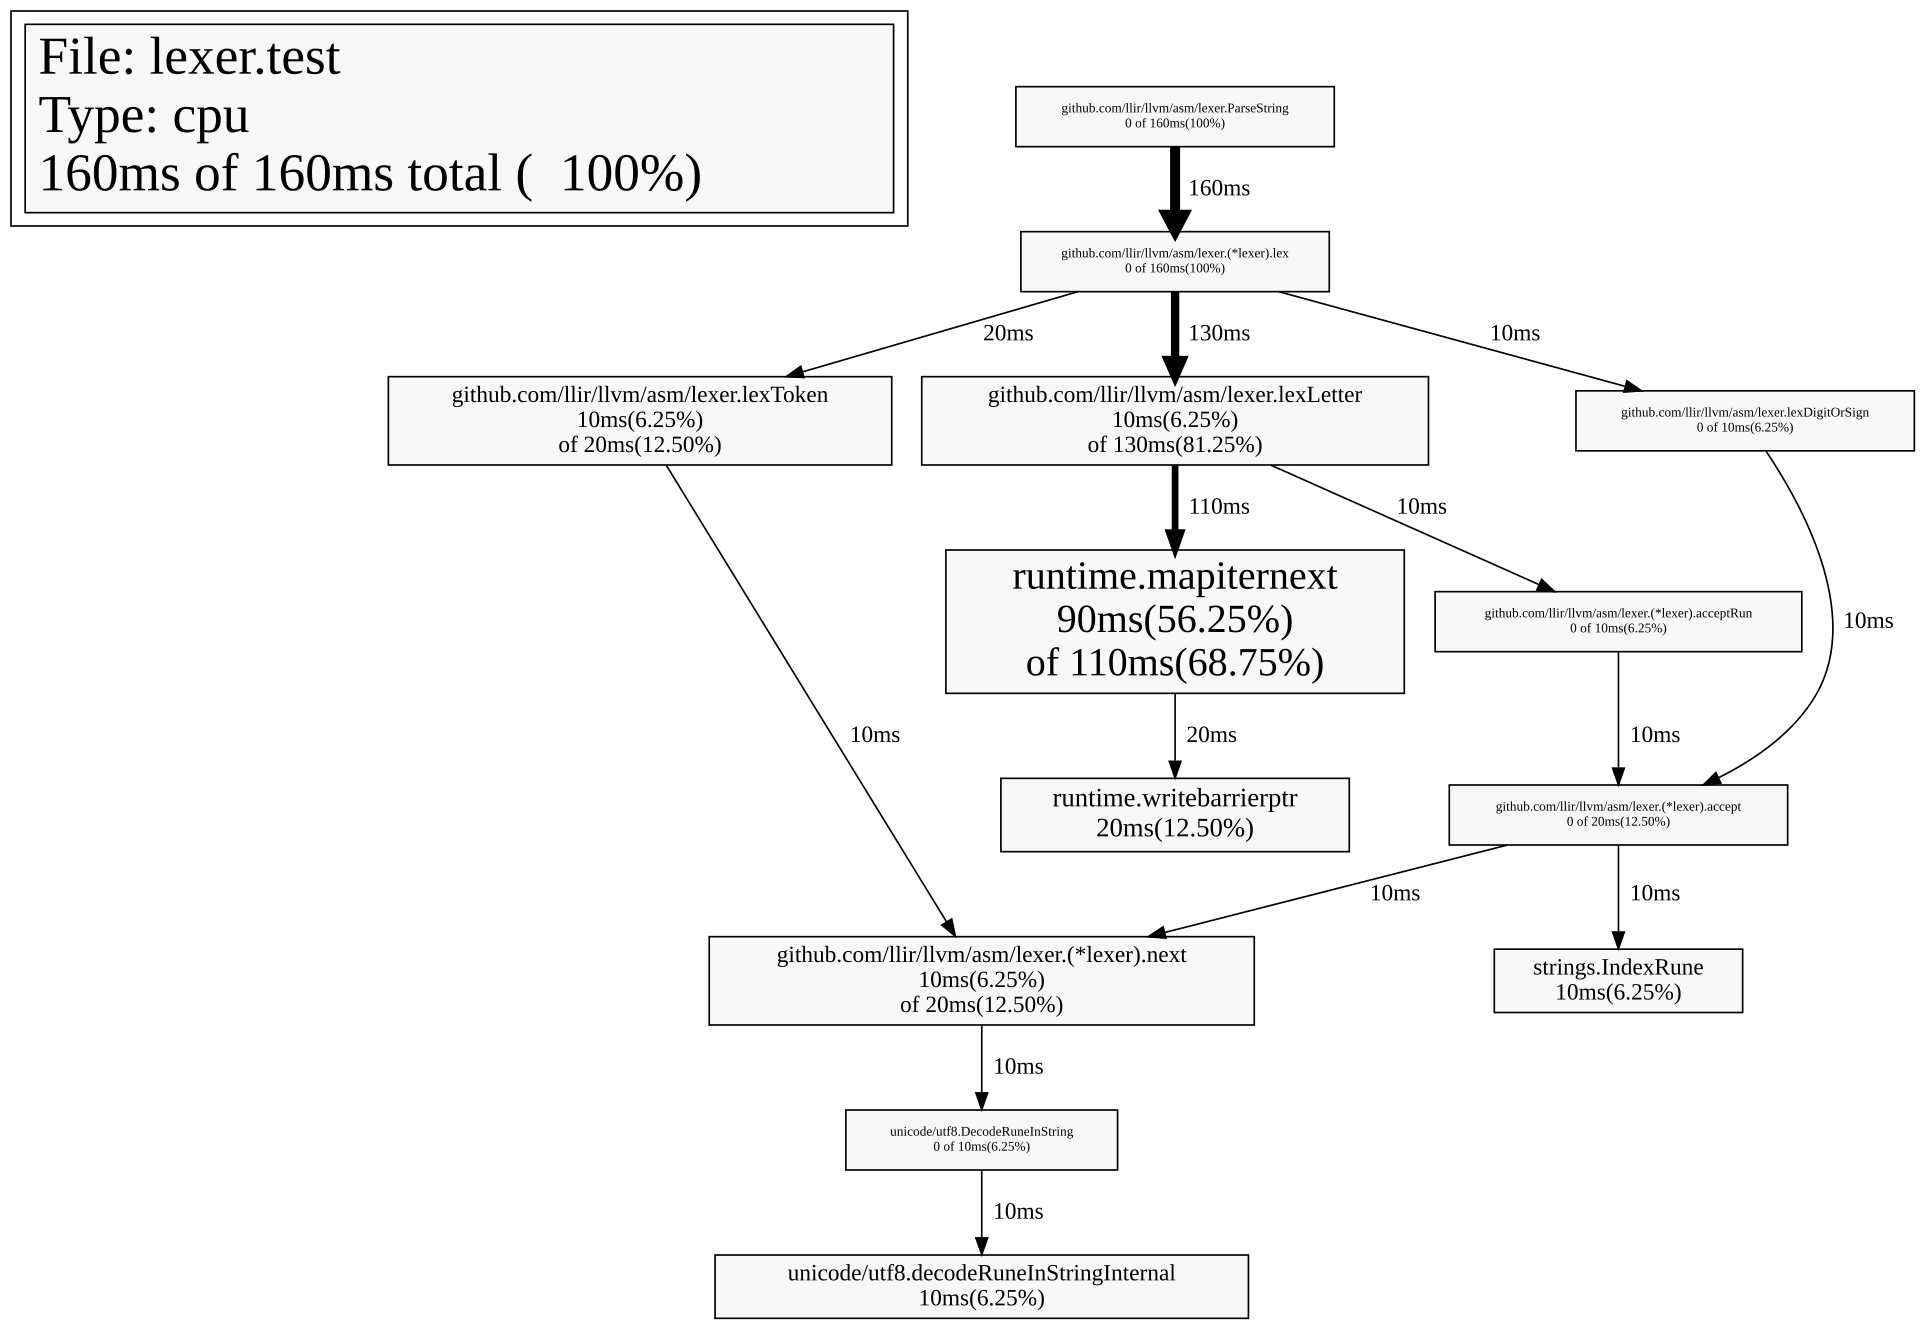
\includegraphics[width=\textwidth]{inc/8_ver/lexer_pprof.png}
		\caption{A major performance bottleneck was located when profiling the LLVM lexer library for the first time. Roughly 70\% of the total execution time was spent doing hash map iterations (i.e. \texttt{runtime.mapiternext}).}
		\label{fig:lexer_pprof}
	\end{center}
\end{figure}
